% vim: set spell spelllang=en tw=100 et sw=4 sts=4 foldmethod=marker foldmarker={{{,}}} :

\documentclass[aspectratio=169,compress,10pt]{beamer}

\usepackage{tikz}
\usepackage{xcolor}
\usepackage{complexity}
\usepackage{hyperref}
\usepackage{microtype}
\usepackage{amsmath}                   % \operatorname
\usepackage{amsfonts}                  % \mathcal
\usepackage{amssymb}                   % \nexists
\usepackage[vlined]{algorithm2e} % algorithms
\usepackage{centernot}
\usepackage{listings}
\usepackage{csquotes}
\usepackage{fancyvrb}
\usepackage{bussproofs}
\usepackage{multicol}
\usepackage{booktabs}
\usepackage{mathtools}
\usepackage{pifont}
\usepackage{marvosym}
\usepackage{cancel}
\usepackage{fontspec}

\usefonttheme{professionalfonts}

\usetikzlibrary{shapes, arrows, shadows, calc, positioning, fit}
\usetikzlibrary{decorations.pathreplacing, decorations.pathmorphing, shapes.misc}
\usetikzlibrary{tikzmark, backgrounds}
\usetikzlibrary{trees, overlay-beamer-styles}
\usetikzlibrary{backgrounds, scopes, graphs, graphs.standard, shapes.geometric}
\usetikzlibrary{shapes.multipart, arrows, arrows.meta, decorations, decorations.markings}

\tikzset{processarrow/.style={->, very thick, decorate, decoration={snake, post length=0.5mm}}}
\tikzset{brace/.style={decorate, decoration={brace}, very thick}}

\definecolor{uofguniversityblue}{rgb}{0, 0.219608, 0.396078}
\definecolor{uofgheather}{rgb}{0.356863, 0.32549, 0.490196}
\definecolor{uofgaquamarine}{rgb}{0.603922, 0.72549, 0.678431}
\definecolor{uofgslate}{rgb}{0.309804, 0.34902, 0.380392}
\definecolor{uofgrose}{rgb}{0.823529, 0.470588, 0.709804}
\definecolor{uofgmocha}{rgb}{0.709804, 0.564706, 0.47451}
\definecolor{uofgsandstone}{rgb}{0.321569, 0.278431, 0.231373}
\definecolor{uofgforest}{rgb}{0, 0.2, 0.129412}
\definecolor{uofglawn}{rgb}{0.517647, 0.741176, 0}
\definecolor{uofgcobalt}{rgb}{0, 0.615686, 0.92549}
\definecolor{uofgturquoise}{rgb}{0, 0.709804, 0.819608}
\definecolor{uofgsunshine}{rgb}{1.0, 0.862745, 0.211765}
\definecolor{uofgpumpkin}{rgb}{1.0, 0.72549, 0.282353}
\definecolor{uofgthistle}{rgb}{0.584314, 0.070588, 0.447059}
\definecolor{uofgrust}{rgb}{0.603922, 0.227451, 0.023529}
\definecolor{uofgburgundy}{rgb}{0.490196, 0.133333, 0.223529}
\definecolor{uofgpillarbox}{rgb}{0.701961, 0.047059, 0}
\definecolor{uofglavendar}{rgb}{0.356863, 0.301961, 0.580392}
\definecolor{uofgleaf}{rgb}{0, 0.517647, 0.239216}

% {{{ theme things
\useoutertheme[footline=authortitle]{miniframes}
\useinnertheme{rectangles}

\setbeamerfont{block title}{size={}}
\setbeamerfont{title}{size=\large,series=\bfseries}
\setbeamerfont{section title}{size=\large,series=\mdseries}
\setbeamerfont{author}{size=\normalsize,series=\mdseries}
\setbeamercolor*{structure}{fg=uofguniversityblue}
\setbeamercolor*{palette primary}{use=structure,fg=black,bg=white}
\setbeamercolor*{palette secondary}{use=structure,fg=white,bg=uofgcobalt}
\setbeamercolor*{palette tertiary}{use=structure,fg=white,bg=uofguniversityblue}
\setbeamercolor*{palette quaternary}{fg=white,bg=black}
\setbeamercolor{block body}{bg=structure!10}
\setbeamercolor{block title}{bg=structure,fg=white}
\setbeamertemplate{blocks}[rounded]
\setbeamercolor*{titlelike}{parent=palette primary}

\beamertemplatenavigationsymbolsempty
\setbeamersize{text margin left=0.5cm}
\setbeamersize{text margin right=0.5cm}

\setbeamertemplate{title page}
{
    \begin{tikzpicture}[remember picture, overlay]
        \node at (current page.north west) {
            \begin{tikzpicture}[remember picture, overlay]
                \fill [fill=uofguniversityblue, anchor=north west] (0, 0) rectangle (\paperwidth, -2.0cm);
            \end{tikzpicture}
        };

        \node (logo) [anchor=north east, shift={(-0.8cm,-0.4cm)}] at (current page.north east) {
            
\includegraphics[keepaspectratio=true,scale=0.5]{../../images/UoG_keyline.pdf}
        };
        \node [anchor=west, xshift=0.8cm] at (current page.west |- logo) {
            \begin{minipage}{0.65\paperwidth}\raggedright
                {\usebeamerfont{title}\usebeamercolor[white]{}\inserttitle}\\[0.2cm]
                {\usebeamerfont{author}\usebeamercolor[white]{}\insertauthor}
            \end{minipage}
        };
    \end{tikzpicture}
}

\setbeamertemplate{section page}
{
    \begin{centering}
        \begin{beamercolorbox}[sep=12pt,center]{part title}
            \usebeamerfont{section title}\insertsection\par
        \end{beamercolorbox}
    \end{centering}
}

\newcommand{\frameofframes}{/}
\newcommand{\setframeofframes}[1]{\renewcommand{\frameofframes}{#1}}

\makeatletter
\setbeamertemplate{footline}
{%
    \begin{beamercolorbox}[colsep=1.5pt]{upper separation line foot}
    \end{beamercolorbox}
    \begin{beamercolorbox}[ht=2.5ex,dp=1.125ex,%
        leftskip=.3cm,rightskip=.3cm plus1fil]{title in head/foot}%
        {\usebeamerfont{title in head/foot}\insertshorttitle}%
        \hspace{0.22\textwidth}%
        {\usebeamerfont{author in head/foot}\insertshortauthor}%
        \hfill%
        {\usebeamerfont{frame number}\usebeamercolor[fg]{frame number}\insertframenumber~\frameofframes~\inserttotalframenumber}
    \end{beamercolorbox}%
    \begin{beamercolorbox}[colsep=1.5pt]{lower separation line foot}
    \end{beamercolorbox}
}

\makeatletter
\setbeamertemplate{mini frame}
{%
  \begin{pgfpicture}{0pt}{0pt}{.04cm}{.04cm}
    \pgfpathcircle{\pgfpoint{0.04cm}{0.04cm}}{0.04cm}
    \pgfusepath{fill,stroke}
  \end{pgfpicture}%
}
\setbeamertemplate{mini frame in current subsection}
{%
  \begin{pgfpicture}{0pt}{0pt}{.04cm}{.04cm}
    \pgfpathcircle{\pgfpoint{0.04cm}{0.04cm}}{0.04cm}
    \pgfsetfillcolor{section in head/foot.bg}
    \pgfusepath{fill,stroke}
  \end{pgfpicture}%
}

\setbeamersize{mini frame size=0.10cm, mini frame offset=0.06cm}
\makeatother

\makeatletter
\newenvironment{nearlyplainframe}[2][]{
    \def\beamer@entrycode{\vspace*{-\headheight}\vspace*{3pt}}
    \setbeamertemplate{headline}
    {%
        \begin{beamercolorbox}[colsep=1.5pt]{upper separation line head}
        \end{beamercolorbox}
        \begin{beamercolorbox}[ht=0.5ex,dp=0.125ex,%
            leftskip=.3cm,rightskip=.3cm plus1fil]{title in head/foot}%
        \end{beamercolorbox}%
        \begin{beamercolorbox}[ht=0.5ex,dp=0.125ex,%
            leftskip=.3cm,rightskip=.3cm plus1fil]{author in head/foot}%
        \end{beamercolorbox}%
        \begin{beamercolorbox}[colsep=1.5pt]{lower separation line head}
        \end{beamercolorbox}
        \vspace*{\headheight}
    }

    \setbeamertemplate{footline}
    {%
        \begin{beamercolorbox}[colsep=1.5pt]{upper separation line foot}
        \end{beamercolorbox}
        \begin{beamercolorbox}[ht=0.5ex,dp=0.125ex,%
            leftskip=.3cm,rightskip=.3cm plus1fil]{author in head/foot}%
        \end{beamercolorbox}%
        \begin{beamercolorbox}[ht=0.5ex,dp=0.125ex,%
            leftskip=.3cm,rightskip=.3cm plus1fil]{title in head/foot}%
        \end{beamercolorbox}%
        \begin{beamercolorbox}[colsep=1.5pt]{lower separation line foot}
        \end{beamercolorbox}
    }

    \begin{frame}[#1]{#2}
    }{
    \end{frame}
}
\makeatother

% }}}

\tikzstyle{state} = [inner sep=1pt]
\tikzstyle{infeasible} = [color=uofgpillarbox]
\tikzstyle{dominated} = [color=uofgcobalt]
\tikzstyle{backwards} = []
\tikzstyle{accept} = [solid, thick]
\tikzstyle{reject} = [dotted, thick]
\tikzstyle{forced} = [color=uofglawn]
\tikzstyle{domination} = [dashed, thick, ->, color=uofgcobalt]

\newcommand{\set}[1]{\{ #1 \}}
\newcommand{\setsize}[1]{{\left|#1\right|}}

\newcommand{\solvernameformat}[1]{\textit{#1}}
\newcommand{\toolformat}[1]{\textit{#1}}
\newcommand{\proofsystemformat}[1]{\textsc{#1}\@}

\newcommand{\veripb}{\toolformat{VeriPB}\xspace}
\renewcommand{\veripb}{\proofsystemformat{VeriPB}\xspace}
\newcommand\veripbid[1]{\alertred{#1}}
\newcommand\veripbConstraint[1]{\alertblue{#1}}

\newcommand{\neighbourhood}{\operatorname{N}}
\newcommand{\vertexset}{\operatorname{V}}
\newcommand{\degree}{\operatorname{deg}}

\author{Arthur Gontier \and Ciaran McCreesh \and Matthew McIlree \and Phil Rodgers}
\title{I Don't Trust Your Algorithms, \\ and You Shouldn't Either}

\begin{document}

{
    \usebackgroundtemplate{
        \tikz[overlay, remember picture]
        \node[at=(current page.south), anchor=south, inner sep=0pt, yshift=-1.4cm]{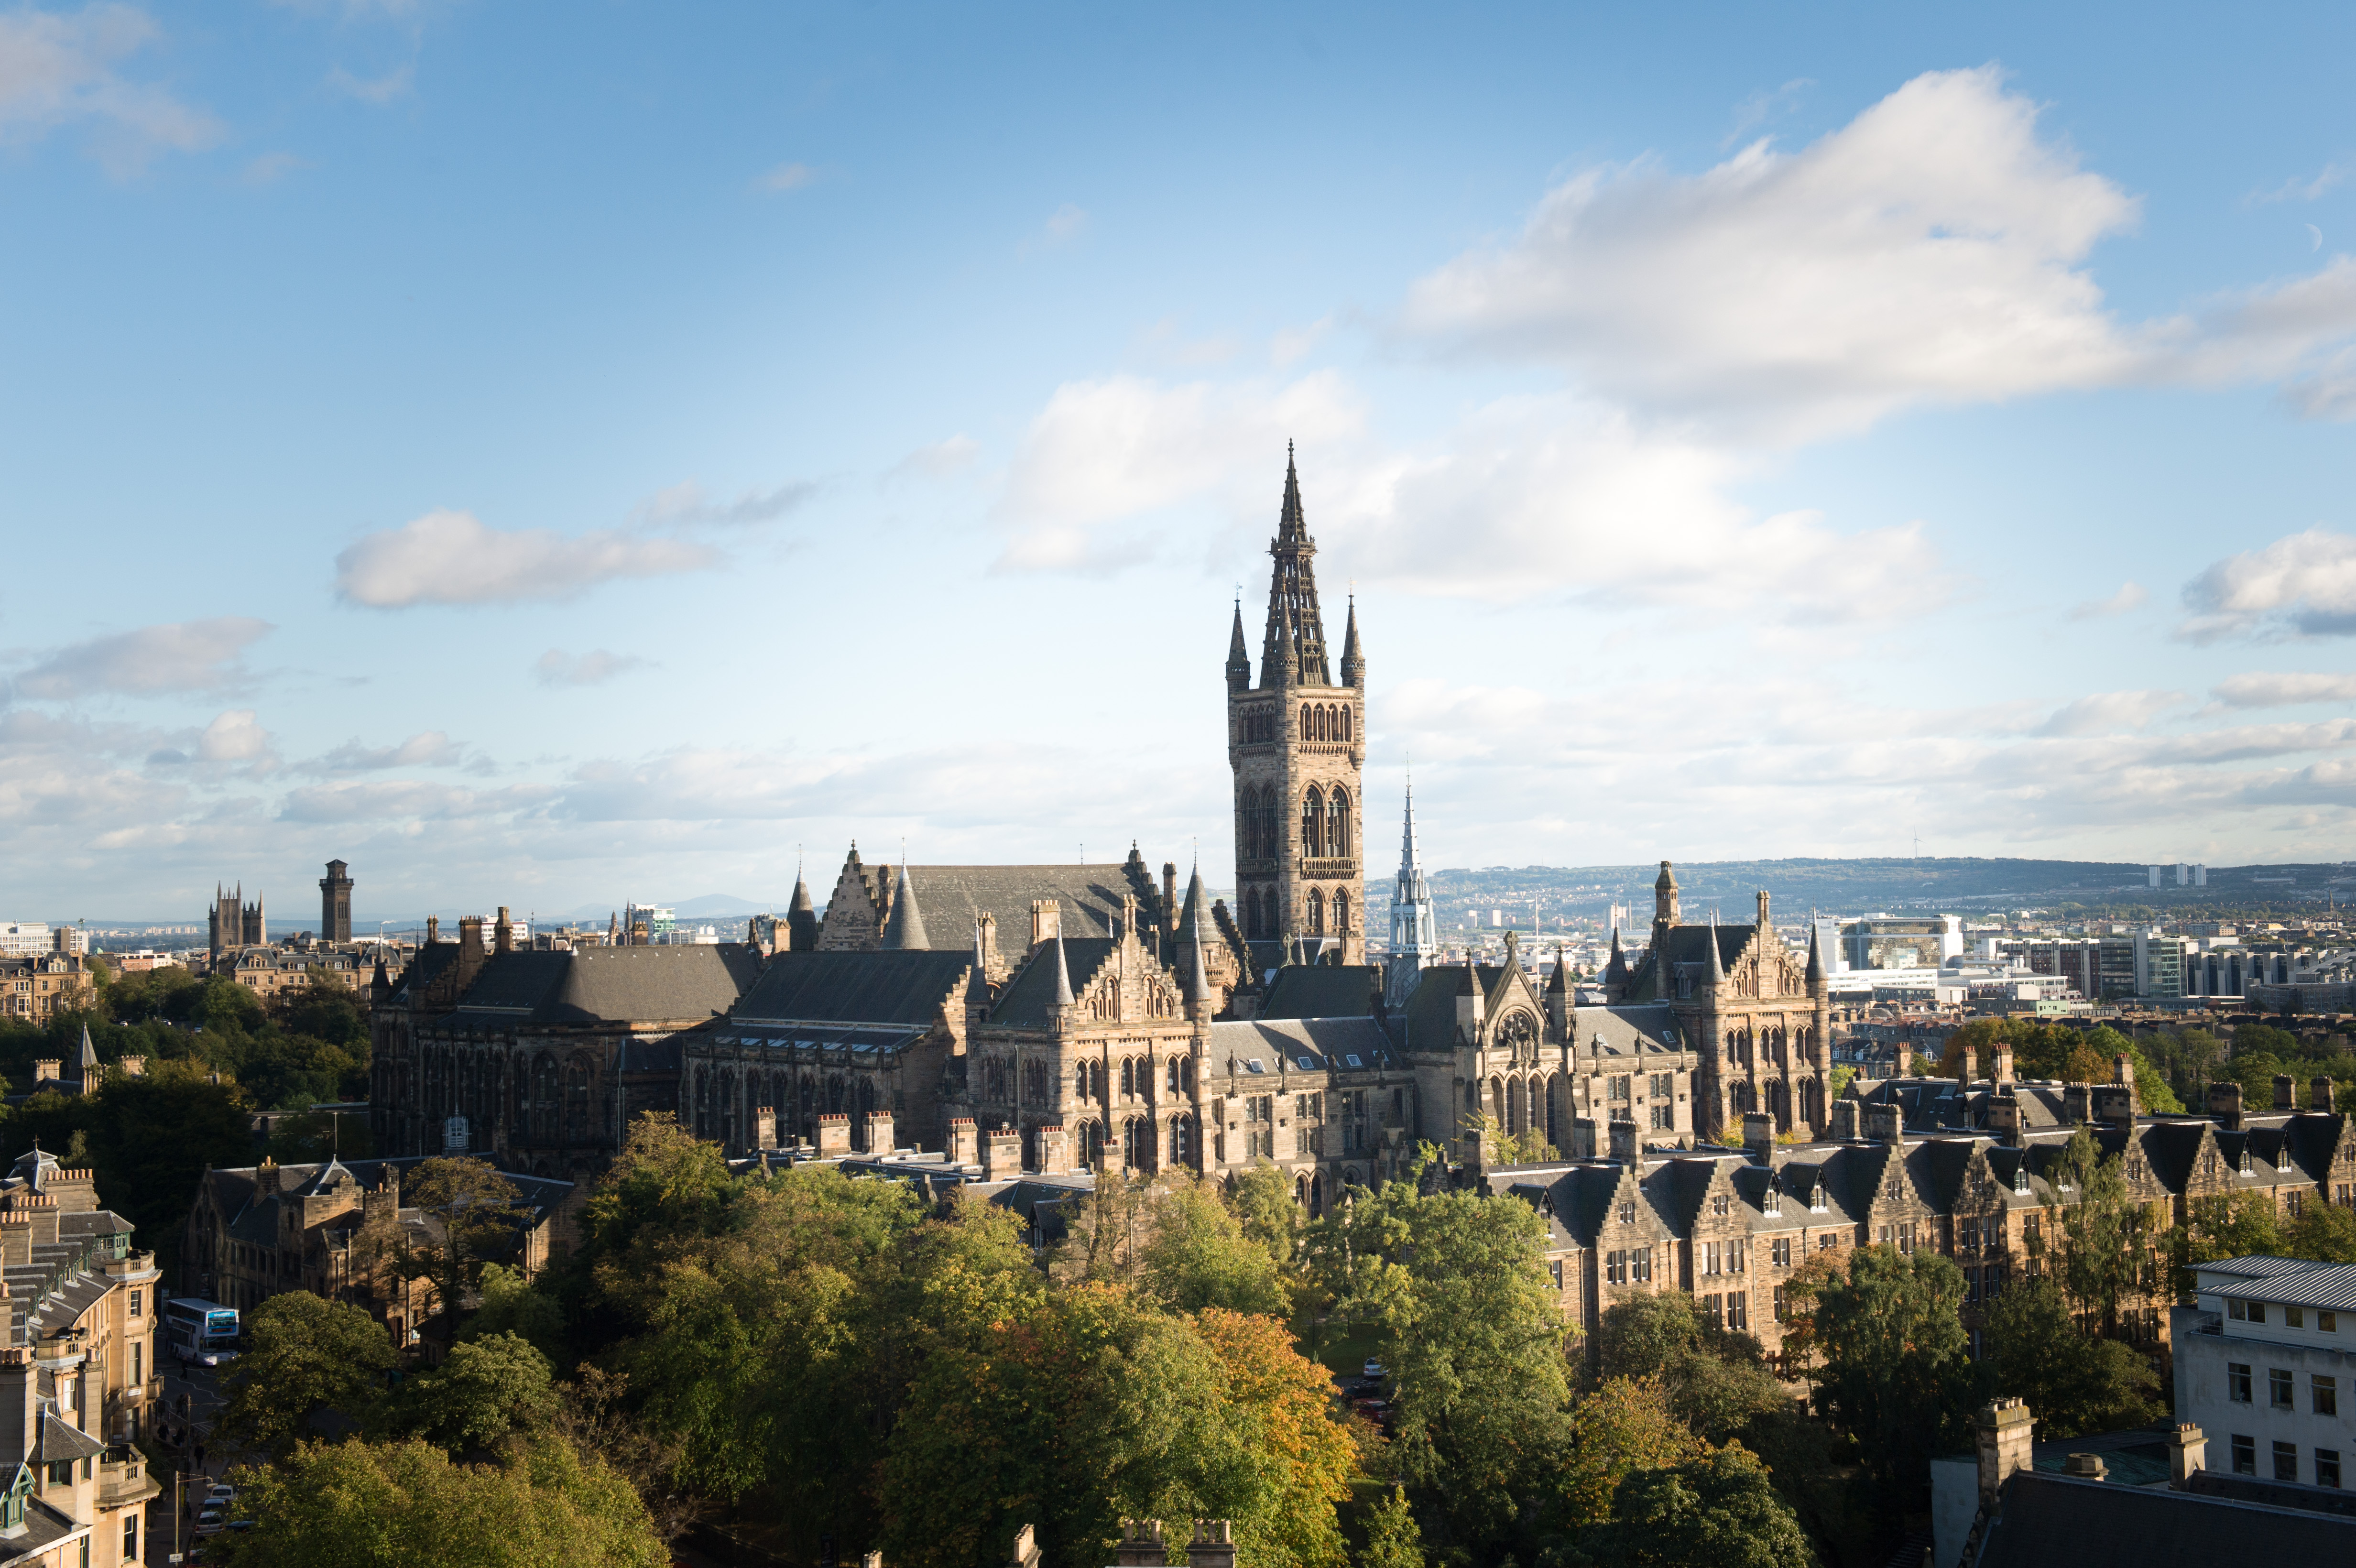
\includegraphics[keepaspectratio=true, width=\paperwidth]{../../images/background.jpg}};
    }
    \begin{frame}[plain,noframenumbering]
        \titlepage
    \end{frame}
}

\begin{frame}{The Slide That Keeps Getting Me Into Trouble}
    2021 MiniZinc challenge: for 1.28\% of instances, wrong solutions were claimed.

    \medskip

    \begin{itemize}
        \item False claims of unsatisfiability.
        \item False claims of optimality.
        \item Infeasible solutions produced.
        \item Not limited to a single solver, problem, or constraint.
        \item Not even consistent---same solver on same hardware and same instance can give
            different results on different runs.
    \end{itemize}

    \medskip \pause
    We've since found similar results across other solving paradigms, and for dedicated solving
    algorithms for hard combinatorial problems.

    \medskip \pause
    Except for CDCL SAT solving!
\end{frame}

\begin{frame}{Proof Logging}
    \vspace*{-1.0em}
    \begin{center}
        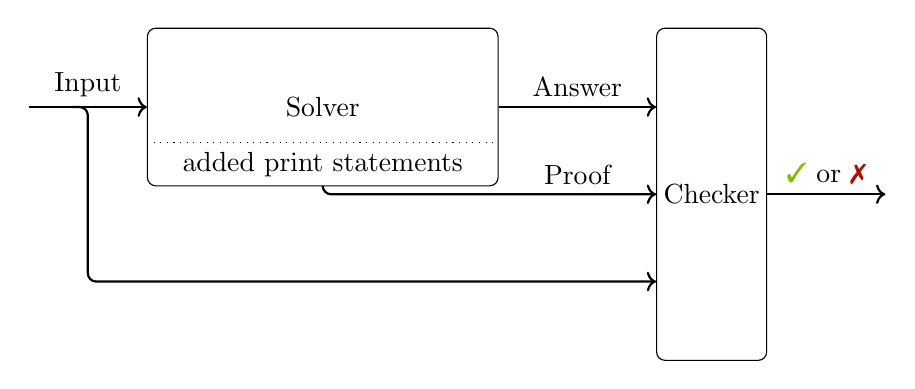
\begin{tikzpicture}
            \node (solver) [inner xsep=5em, inner ysep=2.5em, draw, rounded corners=3pt] { Solver };

            \node (checker) [right=2cm of solver.north east, anchor=north west, inner xsep=0.25em, draw, rounded corners=3pt, minimum height=12em, visible on=<3->] { Checker };

            \node (print) [anchor=south, above=0cm of solver.south, visible on=<2->] { added print statements };
            \draw [dotted, visible on=<2->] (solver.west|-print.north) -- (solver.east|-print.north);

            \draw [->, thick] (solver.east) -- (solver.east -| checker.west)
                coordinate [midway] (solutionmid) node [above, midway] { Answer };

            \draw [->, thick, rounded corners=3pt, visible on=<2->] (solver.south) -- (solver.south |- checker.west)
                -- (checker.west) coordinate [midway] (proofmid);

            \coordinate (prooflabel) at (proofmid-|solutionmid);
            \node [above=0cm of prooflabel, visible on=<2->] { Proof };

            \coordinate [right=1.5cm of checker.east] (verified);
            \draw [->, thick, visible on=<4->] (checker.east) -- (verified) node [above, midway] { \textcolor{uofglawn}{\ding{51}} or \textcolor{uofgpillarbox}{\ding{55}} };

            \coordinate [left=1.5cm of solver.west] (input);
            \draw [->, thick] (input) -- (solver.west) coordinate [midway] (inputmid) node [above, midway] { Input };

            \coordinate (checkerbotleft) at ($(checker.west)+($(checker.west)-(solver.east-|checker.west)$)$);

            \draw [->, thick, rounded corners=3pt, visible on=<3->] ($(inputmid)+(-0.2,0)$) -- (inputmid) -- (inputmid |- checkerbotleft) -- (checkerbotleft);
        \end{tikzpicture}
      \end{center}
    \vspace*{-0.7em}
  \begin{enumerate}
  \item<1->
    Run solver on problem input.
  \item<2->
    Solver also prints out a proof as part of its output.
  \item<3->
    Feed input + solution + proof to proof checker.
  \item<4->
    Verify that proof checker says solution is correct.
  \end{enumerate}
\end{frame}

\begin{frame}[fragile]{What is a Proof?}
     \begin{itemize}
         \item Start with some facts about the problem, which we assume are true.
         \item At each step, derive a new fact from existing facts, in a way that is easily
             checkable if we agree with each previous fact.
         \item Finish by deriving whatever we want to show.
     \end{itemize}
\end{frame}

\begin{frame}{Why This is Hard}
    \begin{itemize}
        \item Proof system must be extremely simple, so we can trust the checker.
        \item But it must also capture rich reasoning that solvers use.
            \begin{itemize}
                \item We don't want a proof system with six hundred rules.
                \item Surprisingly, cutting planes with dominance appears to satisfy both criteria.
            \end{itemize}
        \item Also need to verify that the low-level representation means the same thing as what the
            user cares about.
    \end{itemize}

    \bigskip

    \begin{center}
        \url{https://veripb.org/}
    \end{center}
\end{frame}

\begin{frame}{Where We're Going}
    \begin{center}
        \begin{tikzpicture}
            \node (solver) [ inner xsep=4em, inner ysep=2.5em, draw, rounded corners=3pt] { Solver };
            \node (elaborator) [ right=2cm of solver.north east, anchor=north west, inner
            xsep=0.25em, draw, rounded corners=3pt, minimum height=12em, text width=5em, text centered] {
                \only<1>{Checker}\only<2->{Elaborator, Justifier, and Trimmer} };
            \node (verifiedchecker) [ right=2cm of elaborator.north east, anchor=north west, inner
                xsep=0.25em, draw, rounded corners=3pt, minimum height=8em, text width=4em, text
                centered, yshift=-2cm, visible on=<3->] { Verified Checker };

            \node (print) [anchor=south, above=0cm of solver.south] { added print statements };
            \draw [dotted] (solver.west|-print.north) -- (solver.east|-print.north);

            \draw [->, thick] (solver.east) -- (solver.east -| elaborator.west) coordinate [midway]
            (solutionmid) node [above, midway] { Answer };

            \draw [->, thick, rounded corners=3pt] (solver.south) -- (solver.south |- elaborator.west) -- (elaborator.west) coordinate [midway] (proofmid);

            \coordinate (prooflabel) at (proofmid-|solutionmid); \node [above=0cm of prooflabel] { Proof };

            \coordinate [right=2cm of verifiedchecker.east] (verified);
            \draw [->, thick, visible on=<3>] (verifiedchecker.east) -- (verified)
                node [above, midway] { \textcolor{uofglawn}{\ding{51}} or \textcolor{uofgpillarbox}{\ding{55}} }
                node [below, midway, text centered, text width=5em] { Trusted Answer };
            \draw [->, thick, visible on=<4>] (verifiedchecker.east) -- (verified)
                node [above, midway] { \textcolor{uofglawn}{\ding{51}} or \textcolor{uofgpillarbox}{\ding{55}} }
                node [below, midway, text centered, text width=5em] { Trusted Answer in Domain Language };

            \coordinate [left=1.5cm of solver.west] (input);
            \draw [->, thick] (input) -- (solver.west) coordinate [midway] (inputmid) node [above, midway] { Input };

            \coordinate (verifiedcheckertopleft) at ($(verifiedchecker.west)+($(0cm,1.2cm)$)$);
            \draw [->, thick, visible on=<2->] (elaborator.east |- verifiedcheckertopleft) --
            (verifiedcheckertopleft) node [above, midway, text width=4em, text centered] { Answer };
            \draw [->, thick, visible on=<2->] (elaborator.east |- verifiedchecker.west) -- (verifiedchecker.west) node [above, midway, text width=4em, text centered] { Kernel Proof };

            \coordinate (elaboratorbotleft) at ($(elaborator.west)+($(elaborator.west)-(solver.east-|elaborator.west)$)$);
            \coordinate (verifiedcheckerbotleft) at ($(verifiedchecker.west)+($(0cm,-1.2cm)$)$);

            \coordinate (elaboratortopright) at ($(elaborator.east)+($(verifiedcheckertopleft)-(verifiedchecker.west)$)$);
            \draw [->, thick] (elaboratortopright) -- (elaboratortopright-|verifiedchecker.west)
                node [above, midway] { \textcolor{uofglawn}{\ding{51}} or \textcolor{uofgpillarbox}{\ding{55}} };

            \coordinate (solverstart) at ($(solver.south)!0.75!(solver.south west)$);
            \coordinate (checkerbotleft) at ($(elaborator.west)+($(elaborator.west)-(solver.east-|elaborator.west)$)$);
            \draw [->, thick, rounded corners=3pt] (solverstart) -- (solverstart |- checkerbotleft) -- (checkerbotleft)
            coordinate [midway] (altinputmid);

            \coordinate (encinputlabel) at (altinputmid-|solutionmid);
            \node [above=0cm of encinputlabel, xshift=-0.5cm] { Encoded Input };

            \draw [->, thick, rounded corners=3pt, visible on=<3>] (solverstart) -- (solverstart |- verifiedcheckerbotleft) -- (verifiedcheckerbotleft);
            \draw [->, thick, rounded corners=3pt, visible on=<4>] ($(inputmid)+(-0.2,0)$) --
            (inputmid) -- (inputmid |- verifiedcheckerbotleft) -- (verifiedcheckerbotleft)
            coordinate [midway] (verinputmid);

            \coordinate (verinputlabel) at (verinputmid-|solutionmid);
            \node [above=0cm of verinputlabel, xshift=-0.5cm, visible on=<4>] { Verified Input };
        \end{tikzpicture}
    \end{center}
\end{frame}

{
    \usebackgroundtemplate{
        \tikz[overlay, remember picture]
        \node[at=(current page.south), anchor=south, yshift=-1cm, inner sep=0pt]{\includegraphics[keepaspectratio=true, width=\paperwidth]{../../images/background2.jpg}};
    }

    \begin{frame}[plain,noframenumbering]
        \begin{tikzpicture}[remember picture, overlay]
            \node at (current page.north west) {
                \begin{tikzpicture}[remember picture, overlay]
                    \fill [fill=uofguniversityblue, anchor=north west] (0, 0) rectangle (\paperwidth, -2.0cm);
                \end{tikzpicture}
            };

            \node (logo) [anchor=north east, shift={(-0.8cm,-0.4cm)}] at (current page.north east) {
                
\includegraphics[keepaspectratio=true,scale=0.5]{../../images/UoG_keyline.pdf}
            };

            \node [anchor=west, xshift=0.8cm] at (current page.west |- logo) {
                \begin{minipage}{0.60\paperwidth}\raggedright
                    \textcolor{white}{\url{https://ciaranm.github.io/}} \\[0.3cm]
                    \textcolor{white}{\href{mailto:ciaran.mccreesh@glasgow.ac.uk}{\nolinkurl{ciaran.mccreesh@glasgow.ac.uk}}}
                \end{minipage}
            };
        \end{tikzpicture}

        \begin{tikzpicture}[remember picture, overlay]
            \node [anchor=center, shift={(-0.8cm,-0.4cm)}, fill=white, opacity=0.9, draw, rounded
            corners=3pt, inner sep=0.3cm] at (current page.center) {
                \Huge \url{https://veripb.org/}
            };
        \end{tikzpicture}
    \end{frame}

}

\end{document}

